\documentclass[journal,12pt,twocolumn]{IEEEtran}
%
\usepackage{setspace}
\usepackage{textcomp}
\usepackage{gensymb}
\usepackage{xcolor}
\usepackage{caption}
%\usepackage{subcaption}
%\doublespacing
\singlespacing

\usepackage{graphicx}
\graphicspath{{./images/}}
\usepackage[colorlinks=true, urlcolor=blue, linkcolor=black]{hyperref}
%\usepackage[parfill]{parskip}
%\usepackage{amssymb}
%\usepackage{relsize}
\usepackage[cmex10]{amsmath}
\usepackage{mathtools}
%\usepackage{amsthm}
%\interdisplaylinepenalty=2500
%\savesymbol{iint}
%\usepackage{txfonts}
%\restoresymbol{TXF}{iint}
%\usepackage{wasysym}
\usepackage{amsthm}
\usepackage{mathrsfs}
\usepackage{txfonts}
\usepackage{stfloats}
\usepackage{cite}
\usepackage{cases}
\usepackage{subfig}
%\usepackage{xtab}
\usepackage{hyperref}
\usepackage{longtable}
\usepackage{multirow}
%\usepackage{algorithm}
%\usepackage{algpseudocode}
\usepackage{enumitem}
\usepackage{mathtools}
%\usepackage{eenrc}
%\usepackage[framemethod=tikz]{mdframed}
%\usepackage{hyperref}
\usepackage{listings}
    \usepackage[latin1]{inputenc}                                 %%
    \usepackage{color}                                            %%
    \usepackage{array}                                            %%
    \usepackage{longtable}                                        %%
    \usepackage{calc}                                             %%
    \usepackage{multirow}                                         %%
    \usepackage{hhline}                                           %%
    \usepackage{ifthen}                                           %%
  %optionally (for landscape tables embedded in another document): %%
    \usepackage{lscape}     
\usepackage{tikz}
\usepackage{circuitikz}
\usepackage{karnaugh-map}
\usepackage{pgf}

\usepackage{url}
\def\UrlBreaks{\do\/\do-}



%\usepackage{stmaryrd}


%\usepackage{wasysym}
%\newcounter{MYtempeqncnt}
\DeclareMathOperator*{\Res}{Res}
%\renewcommand{\baselinestretch}{2}
\renewcommand\thesection{\arabic{section}}
\renewcommand\thesubsection{\thesection.\arabic{subsection}}
\renewcommand\thesubsubsection{\thesubsection.\arabic{subsubsection}}

\renewcommand\thesectiondis{\arabic{section}}
\renewcommand\thesubsectiondis{\thesectiondis.\arabic{subsection}}
\renewcommand\thesubsubsectiondis{\thesubsectiondis.\arabic{subsubsection}}



%\surroundwithmdframed[width=\columnwidth]{lstlisting}
\def\inputGnumericTable{}                                 %%
\lstset{
%language=C,
frame=single, 
breaklines=true,
columns=fullflexible
}
 

\begin{document}
%

\theoremstyle{definition}
\newtheorem{theorem}{Theorem}[section]
\newtheorem{problem}{Problem}
\newtheorem{proposition}{Proposition}[section]
\newtheorem{lemma}{Lemma}[section]
\newtheorem{corollary}[theorem]{Corollary}
\newtheorem{example}{Example}[section]
\newtheorem{definition}{Definition}[section]
%\newtheorem{algorithm}{Algorithm}[section]
%\newtheorem{cor}{Corollary}
\newcommand{\BEQA}{\begin{eqnarray}}
\newcommand{\EEQA}{\end{eqnarray}}
\newcommand{\define}{\stackrel{\triangle}{=}}
\vspace{2cm}
\title{ 
Assignment
}

\author{M Shantipriya}


\maketitle
\tableofcontents
%
%\newpage
\section*{\textbf{Question}}

For the given boolean expression f=$\bar{a}$$\bar{b}$$\bar{c}$+$\bar{a}$b$\bar{c}$+a$\bar{b}$$\bar{c}$+abc+ab$\bar{c}$ , the minimized Product of Sum (POS) expression is

\section{\textbf{Components}}
%%%%%%%%%%%%%%%%%%%%%%%%%%%%%%%%%%%%%%%%%%%%%%%%%%%%%%%%%%%%%%%%%%%%%%
%%                                                                  %%
%%  This is the header of a LaTeX2e file exported from Gnumeric.    %%
%%                                                                  %%
%%  This file can be compiled as it stands or included in another   %%
%%  LaTeX document. The table is based on the longtable package so  %%
%%  the longtable options (headers, footers...) can be set in the   %%
%%  preamble section below (see PRAMBLE).                           %%
%%                                                                  %%
%%  To include the file in another, the following two lines must be %%
%%  in the including file:                                          %%
%%        \def\inputGnumericTable{}                                 %%
%%  at the beginning of the file and:                               %%
%%        \input{name-of-this-file.tex}                             %%
%%  where the table is to be placed. Note also that the including   %%
%%  file must use the following packages for the table to be        %%
%%  rendered correctly:                                             %%
%%    \usepackage[latin1]{inputenc}                                 %%
%%    \usepackage{color}                                            %%
%%    \usepackage{array}                                            %%
%%    \usepackage{longtable}                                        %%
%%    \usepackage{calc}                                             %%
%%    \usepackage{multirow}                                         %%
%%    \usepackage{hhline}                                           %%
%%    \usepackage{ifthen}                                           %%
%%  optionally (for landscape tables embedded in another document): %%
%%    \usepackage{lscape}                                           %%
%%                                                                  %%
%%%%%%%%%%%%%%%%%%%%%%%%%%%%%%%%%%%%%%%%%%%%%%%%%%%%%%%%%%%%%%%%%%%%%%



%%  This section checks if we are begin input into another file or  %%
%%  the file will be compiled alone. First use a macro taken from   %%
%%  the TeXbook ex 7.7 (suggestion of Han-Wen Nienhuys).            %%
\def\ifundefined#1{\expandafter\ifx\csname#1\endcsname\relax}


%%  Check for the \def token for inputed files. If it is not        %%
%%  defined, the file will be processed as a standalone and the     %%
%%  preamble will be used.                                          %%
\ifundefined{inputGnumericTable}

%%  We must be able to close or not the document at the end.        %%
	\def\gnumericTableEnd{\end{document}}


%%%%%%%%%%%%%%%%%%%%%%%%%%%%%%%%%%%%%%%%%%%%%%%%%%%%%%%%%%%%%%%%%%%%%%
%%                                                                  %%
%%  This is the PREAMBLE. Change these values to get the right      %%
%%  paper size and other niceties.                                  %%
%%                                                                  %%
%%%%%%%%%%%%%%%%%%%%%%%%%%%%%%%%%%%%%%%%%%%%%%%%%%%%%%%%%%%%%%%%%%%%%%

	\documentclass[12pt%
			  %,landscape%
                    ]{report}
       \usepackage[latin1]{inputenc}
       \usepackage{fullpage}
       \usepackage{color}
       \usepackage{array}
       \usepackage{longtable}
       \usepackage{calc}
       \usepackage{multirow}
       \usepackage{hhline}
       \usepackage{ifthen}

	\begin{document}


%%  End of the preamble for the standalone. The next section is for %%
%%  documents which are included into other LaTeX2e files.          %%
\else

%%  We are not a stand alone document. For a regular table, we will %%
%%  have no preamble and only define the closing to mean nothing.   %%
    \def\gnumericTableEnd{}

%%  If we want landscape mode in an embedded document, comment out  %%
%%  the line above and uncomment the two below. The table will      %%
%%  begin on a new page and run in landscape mode.                  %%
%       \def\gnumericTableEnd{\end{landscape}}
%       \begin{landscape}


%%  End of the else clause for this file being \input.              %%
\fi

%%%%%%%%%%%%%%%%%%%%%%%%%%%%%%%%%%%%%%%%%%%%%%%%%%%%%%%%%%%%%%%%%%%%%%
%%                                                                  %%
%%  The rest is the gnumeric table, except for the closing          %%
%%  statement. Changes below will alter the table's appearance.     %%
%%                                                                  %%
%%%%%%%%%%%%%%%%%%%%%%%%%%%%%%%%%%%%%%%%%%%%%%%%%%%%%%%%%%%%%%%%%%%%%%

\providecommand{\gnumericmathit}[1]{#1} 
%%  Uncomment the next line if you would like your numbers to be in %%
%%  italics if they are italizised in the gnumeric table.           %%
%\renewcommand{\gnumericmathit}[1]{\mathit{#1}}
\providecommand{\gnumericPB}[1]%
{\let\gnumericTemp=\\#1\let\\=\gnumericTemp\hspace{0pt}}
 \ifundefined{gnumericTableWidthDefined}
        \newlength{\gnumericTableWidth}
        \newlength{\gnumericTableWidthComplete}
        \newlength{\gnumericMultiRowLength}
        \global\def\gnumericTableWidthDefined{}
 \fi
%% The following setting protects this code from babel shorthands.  %%
 \ifthenelse{\isundefined{\languageshorthands}}{}{\languageshorthands{english}}
%%  The default table format retains the relative column widths of  %%
%%  gnumeric. They can easily be changed to c, r or l. In that case %%
%%  you may want to comment out the next line and uncomment the one %%
%%  thereafter                                                      %%
\providecommand\gnumbox{\makebox[0pt]}
%%\providecommand\gnumbox[1][]{\makebox}

%% to adjust positions in multirow situations                       %%
\setlength{\bigstrutjot}{\jot}
\setlength{\extrarowheight}{\doublerulesep}

%%  The \setlongtables command keeps column widths the same across  %%
%%  pages. Simply comment out next line for varying column widths.  %%
\setlongtables

\setlength\gnumericTableWidth{%
	100pt+%
	50pt+%
	50pt+%
0pt}
\def\gumericNumCols{3}
\setlength\gnumericTableWidthComplete{\gnumericTableWidth+%
         \tabcolsep*\gumericNumCols*2+\arrayrulewidth*\gumericNumCols}
\ifthenelse{\lengthtest{\gnumericTableWidthComplete > \linewidth}}%
         {\def\gnumericScale{\ratio{\linewidth-%
                        \tabcolsep*\gumericNumCols*2-%
                        \arrayrulewidth*\gumericNumCols}%
{\gnumericTableWidth}}}%
{\def\gnumericScale{1}}

%%%%%%%%%%%%%%%%%%%%%%%%%%%%%%%%%%%%%%%%%%%%%%%%%%%%%%%%%%%%%%%%%%%%%%
%%                                                                  %%
%% The following are the widths of the various columns. We are      %%
%% defining them here because then they are easier to change.       %%
%% Depending on the cell formats we may use them more than once.    %%
%%                                                                  %%
%%%%%%%%%%%%%%%%%%%%%%%%%%%%%%%%%%%%%%%%%%%%%%%%%%%%%%%%%%%%%%%%%%%%%%

\ifthenelse{\isundefined{\gnumericColA}}{\newlength{\gnumericColA}}{}\settowidth{\gnumericColA}{\begin{tabular}{@{}p{100pt*\gnumericScale}@{}}x\end{tabular}}
\ifthenelse{\isundefined{\gnumericColB}}{\newlength{\gnumericColB}}{}\settowidth{\gnumericColB}{\begin{tabular}{@{}p{50pt*\gnumericScale}@{}}x\end{tabular}}
\ifthenelse{\isundefined{\gnumericColC}}{\newlength{\gnumericColC}}{}\settowidth{\gnumericColC}{\begin{tabular}{@{}p{50pt*\gnumericScale}@{}}x\end{tabular}}

\begin{tabular}[c]{%
	b{\gnumericColA}%
	b{\gnumericColB}%
	b{\gnumericColC}%
	}

%%%%%%%%%%%%%%%%%%%%%%%%%%%%%%%%%%%%%%%%%%%%%%%%%%%%%%%%%%%%%%%%%%%%%%
%%  The longtable options. (Caption, headers... see Goosens, p.124) %%
%	\caption{The Table Caption.}             \\	%
% \hline	% Across the top of the table.
%%  The rest of these options are table rows which are placed on    %%
%%  the first, last or every page. Use \multicolumn if you want.    %%

%%  Header for the first page.                                      %%
%	\multicolumn{3}{c}{The First Header} \\ \hline 
%	\multicolumn{1}{c}{colTag}	%Column 1
%	&\multicolumn{1}{c}{colTag}	%Column 2
%	&\multicolumn{1}{c}{colTag}	\\ \hline %Last column
%	\endfirsthead

%%  The running header definition.                                  %%
%	\hline
%	\multicolumn{3}{l}{\ldots\small\slshape continued} \\ \hline
%	\multicolumn{1}{c}{colTag}	%Column 1
%	&\multicolumn{1}{c}{colTag}	%Column 2
%	&\multicolumn{1}{c}{colTag}	\\ \hline %Last column
%	\endhead

%%  The running footer definition.                                  %%
%	\hline
%	\multicolumn{3}{r}{\small\slshape continued\ldots} \\
%	\endfoot

%%  The ending footer definition.                                   %%
%	\multicolumn{3}{c}{That's all folks} \\ \hline 
%	\endlastfoot
%%%%%%%%%%%%%%%%%%%%%%%%%%%%%%%%%%%%%%%%%%%%%%%%%%%%%%%%%%%%%%%%%%%%%%

\hhline{|-|-|-}
	 \multicolumn{1}{|p{\gnumericColA}|}%
	{\gnumericPB{\centering}\textbf{Component}}
	&\multicolumn{1}{p{\gnumericColB}|}%
	{\gnumericPB{\centering}\textbf{Value}}
	&\multicolumn{1}{p{\gnumericColC}|}%
	{\gnumericPB{\centering}\textbf{Quantity}}
\\
\hhline{|---|}
	 \multicolumn{1}{|p{\gnumericColA}|}%
	{\gnumericPB{\centering}Resistor}
	&\multicolumn{1}{p{\gnumericColB}|}%
	{\gnumericPB{\centering}220 Ohm}
	&\multicolumn{1}{p{\gnumericColC}|}%
	{\gnumericPB{\centering}1}
\\
\hhline{|---|}
	 \multicolumn{1}{|p{\gnumericColA}|}%
	{\gnumericPB{\centering}Arduino}
	&\multicolumn{1}{p{\gnumericColB}|}%
	{\gnumericPB{\centering}UNO}
	&\multicolumn{1}{p{\gnumericColC}|}%
	{\gnumericPB{\centering}1}
\\
\hhline{|---|}
	 \multicolumn{1}{|p{\gnumericColA}|}%
	{\gnumericPB{\centering}Seven Segment Display}
	&\multicolumn{1}{p{\gnumericColB}|}%
	{}
	&\multicolumn{1}{p{\gnumericColC}|}%
	{\gnumericPB{\centering}1}
\\
\hhline{|---|}
	 \multicolumn{1}{|p{\gnumericColA}|}%
	{\gnumericPB{\centering}Decoder}
	&\multicolumn{1}{p{\gnumericColB}|}%
	{\gnumericPB{\centering}7447}
	&\multicolumn{1}{p{\gnumericColC}|}%
	{\gnumericPB{\centering}1}
\\
\hhline{|---|}
	 \multicolumn{1}{|p{\gnumericColA}|}%
	{\gnumericPB{\centering}\gnumbox{Jumper Wires}}
	&\multicolumn{1}{p{\gnumericColB}|}%
	{\gnumericPB{\centering}\gnumbox{M-M}}
	&\multicolumn{1}{p{\gnumericColC}|}%
	{\gnumericPB{\centering}\gnumbox{20}}
\\
\hhline{|---|}
	 \multicolumn{1}{|p{\gnumericColA}|}%
	{\gnumericPB{\centering}\gnumbox{Breadboard}}
	&\multicolumn{1}{p{\gnumericColB}|}%
	{}
	&\multicolumn{1}{p{\gnumericColC}|}%
	{\gnumericPB{\centering}\gnumbox{1}}
\\
\hhline{|-|-|-|}
\end{tabular}

\ifthenelse{\isundefined{\languageshorthands}}{}{\languageshorthands{\languagename}}
\gnumericTableEnd
\begin{table}[!h]
\centering
\caption{}
\label{table:7447_disp}
\end{table}

\begin{figure}[!h]
2.The figure given below is the pin diagram of Seven Segment Display.\\
\begin{center}
\resizebox {0.4\columnwidth} {!} {


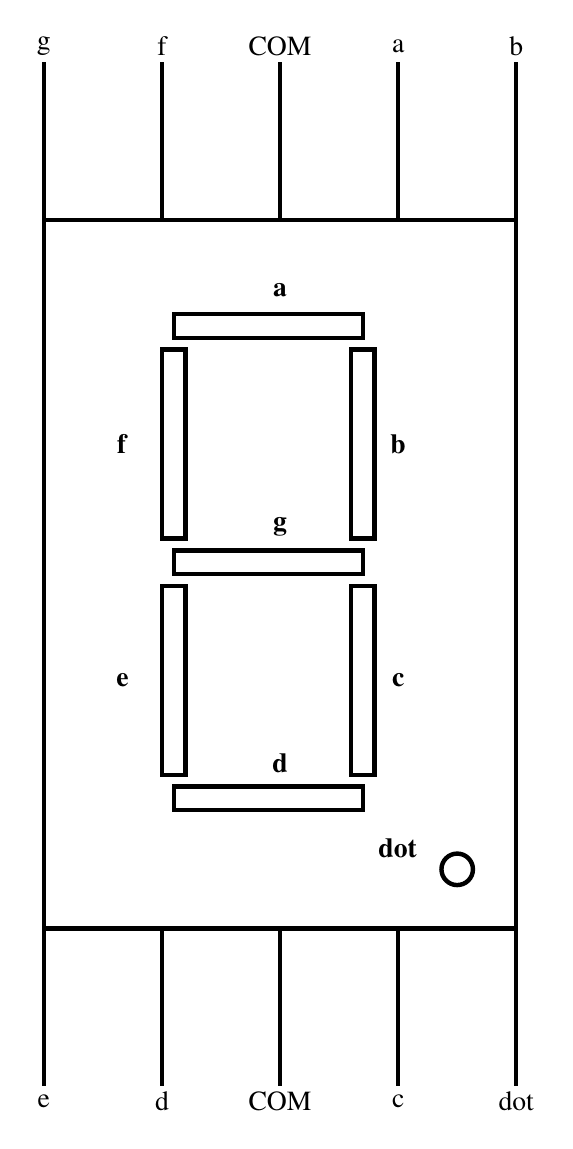
\begin{tikzpicture}
  [
    scale=1,
    >=stealth,
    point/.style = {draw, circle,  fill = black, inner sep = 0.5pt},
    dot/.style   = {draw, circle,  fill = black, inner sep = .2pt},
  ]

%Vertices of the main display rectangle
\def \xmin{0}
\def \xmax{6}
\def \ymin{0}
\def \ymax{-9}

%Number of pins on a side
\def \n{5}
\def \k{1.6}

%Draw the display rectangle
\draw[ultra thick] (\xmin,\ymin)rectangle (\xmax,\ymax);

%Define height of pins and their separation
\def \height{2}
\pgfmathsetmacro{\wid}{(\xmax-\xmin)/(\n-1)}

%Defining y axis divisions
\pgfmathsetmacro{\ywid}{(\ymin-\ymax)/(\n-2)}

\foreach \i in {0,...,4}
{
\draw[ultra thick] (\xmin + \i*\wid, \ymin) -- (\xmin + \i*\wid, \ymin + \height); 
\draw[ultra thick] (\xmin + \i*\wid, \ymax) -- (\xmin + \i*\wid, \ymax -\height); 
}
%%
%%%
\foreach [count=\i] \j in {g,f,COM,a,b}{
            \node (\i) at ( -1.5 + \i*\wid,\height+0.2) {\j} ;
            }
\foreach [count=\i] \j in {e,d,COM,c,dot}{
            \node (\i) at ( -1.5 + \i*\wid,\ymax -\height-0.2) {\j} ;
            }

\foreach [count=\i] \j in {\textbf{a},\textbf{g},\textbf{d}}
{            
\draw[ultra thick] (\xmin+1.1*\wid,{\ymin-(\i-0.5)*\ywid} ) rectangle +(\k*\wid,0.3 );
\node (\i) at ( \xmin + 2*\wid,{\ymin-(\i-0.7)*\ywid}) {\j} ;
}
\foreach [count=\i] \j in {\textbf{f},\textbf{e}}
{            
\draw[ultra thick] (\xmin+\wid,{\ymin-(\i+0.35)*\ywid} ) rectangle +(0.3,\k*\wid );
\node (\i) at ( \xmin + \wid-0.5,{\ymin-(\i-0.05)*\ywid}) {\j} ;
}
\foreach [count=\i] \j in {\textbf{b},\textbf{c}}
{            
\draw[ultra thick] (\xmin+2.6*\wid,{\ymin-(\i+0.35)*\ywid } ) rectangle +(0.3,\k*\wid );
\node (\i) at ( \xmin + 3*\wid,{\ymin-(\i-0.05)*\ywid}) {\j} ;
}


%
\draw[ultra thick] (\xmax - 0.5*\wid,{\ymax+0.25*\ywid}) circle [radius=0.2];
\draw[ultra thick](\xmax - 0.5*\wid,{\ymax+0.25*\ywid}) node[sloped, anchor=center, above, text width=2.0cm]{\textbf{dot}};    
\end{tikzpicture}
}
\end{center}

\caption{}
\label{fig:sevenseg}
\end{figure}

\begin{table}[!h]
1.The table given below is the connections between 7447 BCD Decoder and Seven Segment Display\\
\centering
%%%%%%%%%%%%%%%%%%%%%%%%%%%%%%%%%%%%%%%%%%%%%%%%%%%%%%%%%%%%%%%%%%%%%%
%%                                                                  %%
%%  This is the header of a LaTeX2e file exported from Gnumeric.    %%
%%                                                                  %%
%%  This file can be compiled as it stands or included in another   %%
%%  LaTeX document. The table is based on the longtable package so  %%
%%  the longtable options (headers, footers...) can be set in the   %%
%%  preamble section below (see PRAMBLE).                           %%
%%                                                                  %%
%%  To include the file in another, the following two lines must be %%
%%  in the including file:                                          %%
%%        \def\inputGnumericTable{}                                 %%
%%  at the beginning of the file and:                               %%
%%        \input{name-of-this-file.tex}                             %%
%%  where the table is to be placed. Note also that the including   %%
%%  file must use the following packages for the table to be        %%
%%  rendered correctly:                                             %%
%%    \usepackage[latin1]{inputenc}                                 %%
%%    \usepackage{color}                                            %%
%%    \usepackage{array}                                            %%
%%    \usepackage{longtable}                                        %%
%%    \usepackage{calc}                                             %%
%%    \usepackage{multirow}                                         %%
%%    \usepackage{hhline}                                           %%
%%    \usepackage{ifthen}                                           %%
%%  optionally (for landscape tables embedded in another document): %%
%%    \usepackage{lscape}                                           %%
%%                                                                  %%
%%%%%%%%%%%%%%%%%%%%%%%%%%%%%%%%%%%%%%%%%%%%%%%%%%%%%%%%%%%%%%%%%%%%%%



%%  This section checks if we are begin input into another file or  %%
%%  the file will be compiled alone. First use a macro taken from   %%
%%  the TeXbook ex 7.7 (suggestion of Han-Wen Nienhuys).            %%
\def\ifundefined#1{\expandafter\ifx\csname#1\endcsname\relax}


%%  Check for the \def token for inputed files. If it is not        %%
%%  defined, the file will be processed as a standalone and the     %%
%%  preamble will be used.                                          %%
\ifundefined{inputGnumericTable}

%%  We must be able to close or not the document at the end.        %%
	\def\gnumericTableEnd{\end{document}}


%%%%%%%%%%%%%%%%%%%%%%%%%%%%%%%%%%%%%%%%%%%%%%%%%%%%%%%%%%%%%%%%%%%%%%
%%                                                                  %%
%%  This is the PREAMBLE. Change these values to get the right      %%
%%  paper size and other niceties.                                  %%
%%                                                                  %%
%%%%%%%%%%%%%%%%%%%%%%%%%%%%%%%%%%%%%%%%%%%%%%%%%%%%%%%%%%%%%%%%%%%%%%

	\documentclass[12pt%
			  %,landscape%
                    ]{report}
       \usepackage[latin1]{inputenc}
       \usepackage{fullpage}
       \usepackage{color}
       \usepackage{array}
       \usepackage{longtable}
       \usepackage{calc}
       \usepackage{multirow}
       \usepackage{hhline}
       \usepackage{ifthen}

	\begin{document}


%%  End of the preamble for the standalone. The next section is for %%
%%  documents which are included into other LaTeX2e files.          %%
\else

%%  We are not a stand alone document. For a regular table, we will %%
%%  have no preamble and only define the closing to mean nothing.   %%
    \def\gnumericTableEnd{}

%%  If we want landscape mode in an embedded document, comment out  %%
%%  the line above and uncomment the two below. The table will      %%
%%  begin on a new page and run in landscape mode.                  %%
%       \def\gnumericTableEnd{\end{landscape}}
%       \begin{landscape}


%%  End of the else clause for this file being \input.              %%
\fi

%%%%%%%%%%%%%%%%%%%%%%%%%%%%%%%%%%%%%%%%%%%%%%%%%%%%%%%%%%%%%%%%%%%%%%
%%                                                                  %%
%%  The rest is the gnumeric table, except for the closing          %%
%%  statement. Changes below will alter the table's appearance.     %%
%%                                                                  %%
%%%%%%%%%%%%%%%%%%%%%%%%%%%%%%%%%%%%%%%%%%%%%%%%%%%%%%%%%%%%%%%%%%%%%%

\providecommand{\gnumericmathit}[1]{#1} 
%%  Uncomment the next line if you would like your numbers to be in %%
%%  italics if they are italizised in the gnumeric table.           %%
%\renewcommand{\gnumericmathit}[1]{\mathit{#1}}
\providecommand{\gnumericPB}[1]%
{\let\gnumericTemp=\\#1\let\\=\gnumericTemp\hspace{0pt}}
 \ifundefined{gnumericTableWidthDefined}
        \newlength{\gnumericTableWidth}
        \newlength{\gnumericTableWidthComplete}
        \newlength{\gnumericMultiRowLength}
        \global\def\gnumericTableWidthDefined{}
 \fi
%% The following setting protects this code from babel shorthands.  %%
 \ifthenelse{\isundefined{\languageshorthands}}{}{\languageshorthands{english}}
%%  The default table format retains the relative column widths of  %%
%%  gnumeric. They can easily be changed to c, r or l. In that case %%
%%  you may want to comment out the next line and uncomment the one %%
%%  thereafter                                                      %%
\providecommand\gnumbox{\makebox[0pt]}
%%\providecommand\gnumbox[1][]{\makebox}

%% to adjust positions in multirow situations                       %%
\setlength{\bigstrutjot}{\jot}
\setlength{\extrarowheight}{\doublerulesep}

%%  The \setlongtables command keeps column widths the same across  %%
%%  pages. Simply comment out next line for varying column widths.  %%
\setlongtables

\setlength\gnumericTableWidth{%
	51pt+%
	10pt+%
	10pt+%
	10pt+%
	10pt+%
	10pt+%
	8pt+%
	10pt+%
0pt}
\def\gumericNumCols{8}
\setlength\gnumericTableWidthComplete{\gnumericTableWidth+%
         \tabcolsep*\gumericNumCols*2+\arrayrulewidth*\gumericNumCols}
\ifthenelse{\lengthtest{\gnumericTableWidthComplete > \linewidth}}%
         {\def\gnumericScale{\ratio{\linewidth-%
                        \tabcolsep*\gumericNumCols*2-%
                        \arrayrulewidth*\gumericNumCols}%
{\gnumericTableWidth}}}%
{\def\gnumericScale{1}}

%%%%%%%%%%%%%%%%%%%%%%%%%%%%%%%%%%%%%%%%%%%%%%%%%%%%%%%%%%%%%%%%%%%%%%
%%                                                                  %%
%% The following are the widths of the various columns. We are      %%
%% defining them here because then they are easier to change.       %%
%% Depending on the cell formats we may use them more than once.    %%
%%                                                                  %%
%%%%%%%%%%%%%%%%%%%%%%%%%%%%%%%%%%%%%%%%%%%%%%%%%%%%%%%%%%%%%%%%%%%%%%

\ifthenelse{\isundefined{\gnumericColA}}{\newlength{\gnumericColA}}{}\settowidth{\gnumericColA}{\begin{tabular}{@{}p{51pt*\gnumericScale}@{}}x\end{tabular}}
\ifthenelse{\isundefined{\gnumericColB}}{\newlength{\gnumericColB}}{}\settowidth{\gnumericColB}{\begin{tabular}{@{}p{10pt*\gnumericScale}@{}}x\end{tabular}}
\ifthenelse{\isundefined{\gnumericColC}}{\newlength{\gnumericColC}}{}\settowidth{\gnumericColC}{\begin{tabular}{@{}p{10pt*\gnumericScale}@{}}x\end{tabular}}
\ifthenelse{\isundefined{\gnumericColD}}{\newlength{\gnumericColD}}{}\settowidth{\gnumericColD}{\begin{tabular}{@{}p{10pt*\gnumericScale}@{}}x\end{tabular}}
\ifthenelse{\isundefined{\gnumericColE}}{\newlength{\gnumericColE}}{}\settowidth{\gnumericColE}{\begin{tabular}{@{}p{10pt*\gnumericScale}@{}}x\end{tabular}}
\ifthenelse{\isundefined{\gnumericColF}}{\newlength{\gnumericColF}}{}\settowidth{\gnumericColF}{\begin{tabular}{@{}p{10pt*\gnumericScale}@{}}x\end{tabular}}
\ifthenelse{\isundefined{\gnumericColG}}{\newlength{\gnumericColG}}{}\settowidth{\gnumericColG}{\begin{tabular}{@{}p{8pt*\gnumericScale}@{}}x\end{tabular}}
\ifthenelse{\isundefined{\gnumericColH}}{\newlength{\gnumericColH}}{}\settowidth{\gnumericColH}{\begin{tabular}{@{}p{10pt*\gnumericScale}@{}}x\end{tabular}}

\begin{tabular}[c]{%
	b{\gnumericColA}%
	b{\gnumericColB}%
	b{\gnumericColC}%
	b{\gnumericColD}%
	b{\gnumericColE}%
	b{\gnumericColF}%
	b{\gnumericColG}%
	b{\gnumericColH}%
	}

%%%%%%%%%%%%%%%%%%%%%%%%%%%%%%%%%%%%%%%%%%%%%%%%%%%%%%%%%%%%%%%%%%%%%%
%%  The longtable options. (Caption, headers... see Goosens, p.124) %%
%	\caption{The Table Caption.}             \\	%
% \hline	% Across the top of the table.
%%  The rest of these options are table rows which are placed on    %%
%%  the first, last or every page. Use \multicolumn if you want.    %%

%%  Header for the first page.                                      %%
%	\multicolumn{8}{c}{The First Header} \\ \hline 
%	\multicolumn{1}{c}{colTag}	%Column 1
%	&\multicolumn{1}{c}{colTag}	%Column 2
%	&\multicolumn{1}{c}{colTag}	%Column 3
%	&\multicolumn{1}{c}{colTag}	%Column 4
%	&\multicolumn{1}{c}{colTag}	%Column 5
%	&\multicolumn{1}{c}{colTag}	%Column 6
%	&\multicolumn{1}{c}{colTag}	%Column 7
%	&\multicolumn{1}{c}{colTag}	\\ \hline %Last column
%	\endfirsthead

%%  The running header definition.                                  %%
%	\hline
%	\multicolumn{8}{l}{\ldots\small\slshape continued} \\ \hline
%	\multicolumn{1}{c}{colTag}	%Column 1
%	&\multicolumn{1}{c}{colTag}	%Column 2
%	&\multicolumn{1}{c}{colTag}	%Column 3
%	&\multicolumn{1}{c}{colTag}	%Column 4
%	&\multicolumn{1}{c}{colTag}	%Column 5
%	&\multicolumn{1}{c}{colTag}	%Column 6
%	&\multicolumn{1}{c}{colTag}	%Column 7
%	&\multicolumn{1}{c}{colTag}	\\ \hline %Last column
%	\endhead

%%  The running footer definition.                                  %%
%	\hline
%	\multicolumn{8}{r}{\small\slshape continued\ldots} \\
%	\endfoot

%%  The ending footer definition.                                   %%
%	\multicolumn{8}{c}{That's all folks} \\ \hline 
%	\endlastfoot
%%%%%%%%%%%%%%%%%%%%%%%%%%%%%%%%%%%%%%%%%%%%%%%%%%%%%%%%%%%%%%%%%%%%%%

\hhline{|-|-|-|-|-|-|-|-}
	 \multicolumn{1}{|p{\gnumericColA}|}%
	{\gnumericPB{\centering}\textbf{7447}}
	&\multicolumn{1}{p{\gnumericColB}|}%
	{\gnumericPB{\centering}$\bar{a}$}
	&\multicolumn{1}{p{\gnumericColC}|}%
	{\gnumericPB{\centering}$\bar{b}$}
	&\multicolumn{1}{p{\gnumericColD}|}%
	{\gnumericPB{\centering}\gnumbox{$\bar{c}$}}
	&\multicolumn{1}{p{\gnumericColE}|}%
	{\gnumericPB{\centering}\gnumbox{$\bar{d}$}}
	&\multicolumn{1}{p{\gnumericColF}|}%
	{\gnumericPB{\centering}\gnumbox{$\bar{e}$}}
	&\multicolumn{1}{p{\gnumericColG}|}%
	{\gnumericPB{\centering}\gnumbox{$\bar{f}$}}
	&\multicolumn{1}{p{\gnumericColH}|}%
	{\gnumericPB{\centering}\gnumbox{$\bar{g}$}}
\\
\hhline{|--------|}
	 \multicolumn{1}{|p{\gnumericColA}|}%
	{\gnumericPB{\centering}\textbf{Display}}
	&\multicolumn{1}{p{\gnumericColB}|}%
	{\gnumericPB{\centering}a}
	&\multicolumn{1}{p{\gnumericColC}|}%
	{\gnumericPB{\centering}b}
	&\multicolumn{1}{p{\gnumericColD}|}%
	{\gnumericPB{\centering}\gnumbox{c}}
	&\multicolumn{1}{p{\gnumericColE}|}%
	{\gnumericPB{\centering}\gnumbox{d}}
	&\multicolumn{1}{p{\gnumericColF}|}%
	{\gnumericPB{\centering}\gnumbox{e}}
	&\multicolumn{1}{p{\gnumericColG}|}%
	{\gnumericPB{\centering}\gnumbox{f}}
	&\multicolumn{1}{p{\gnumericColH}|}%
	{\gnumericPB{\centering}\gnumbox{g}}
\\
\hhline{|-|-|-|-|-|-|-|-|}
\end{tabular}

\ifthenelse{\isundefined{\languageshorthands}}{}{\languageshorthands{\languagename}}
\gnumericTableEnd

\caption{}
\label{table:7447_disp}
\end{table}
\begin{figure}[!h]
3.The diagram below shows the pin diagram of 7447 BCD Decoder.The output pins of 7447 is connected to Seven Segment Display using Table 2.
\begin{center}
\resizebox {1.2\columnwidth} {!} {
%\documentclass{standalone}
%\usepackage{tikz}
%\usepackage{amsmath,amssymb}
\makeatletter
\newsavebox\myboxA
\newsavebox\myboxB
\newlength\mylenA
\newcommand*\xoverline[2][0.75]{%
    \sbox{\myboxA}{$\m@th#2$}%
    \setbox\myboxB\null% Phantom box
    \ht\myboxB=\ht\myboxA%
    \dp\myboxB=\dp\myboxA%
    \wd\myboxB=#1\wd\myboxA% Scale phantom
    \sbox\myboxB{$\m@th\overline{\copy\myboxB}$}%  Overlined phantom
    \setlength\mylenA{\the\wd\myboxA}%   calc width diff
    \addtolength\mylenA{-\the\wd\myboxB}%
    \ifdim\wd\myboxB<\wd\myboxA%
       \rlap{\hskip 0.5\mylenA\usebox\myboxB}{\usebox\myboxA}%
    \else
        \hskip -0.5\mylenA\rlap{\usebox\myboxA}{\hskip 0.5\mylenA\usebox\myboxB}%
    \fi}
\makeatother


%\begin{document}
\begin{tikzpicture}[scale=1,
     pin/.style={draw,rectangle,minimum width=2em,font=\small}
     ]
   % Main trick: loop over the label numbers and then adjust their position
   % in the tikzpicture using evaluate to calculate \y=y-coordinate of pin

   \foreach \i/\desc [evaluate=\i  as \x using (\i+4.8 )]
      in {1/\tiny{B},
          2/\tiny{C},
          3/\tiny{\xoverline{LT}},
          4/\tiny{\xoverline{BI/RBO}},
          5/\tiny{\xoverline{RBI}},
          6/\tiny{D},
          7/\tiny{A},
          8/\tiny{GND}}
   {
     \draw node[pin,anchor=east,rotate=360] at (\x,-0.233){\small$\i$};
     \node[align=right,anchor=east,rotate=360] at (\x,-.8){\desc};
   }
  
   \foreach \i/\desc [evaluate=\i as \x using (21.1-\i)]
      in { 9/\xoverline{e},
          10/\xoverline{d},
          11/\xoverline{c},
          12/\xoverline{b},
          13/\xoverline{a},
          14/\xoverline{g},
          15/\xoverline{f},
          16/{V$_{\text{CC}}$}}
   {
     \draw node[pin,anchor=west,rotate=360] at (\x,3.22){\small$\i$};
     \node[align=right,anchor=west,rotate=360] at (\x,3.8){\desc};
   }
   \draw
      (5,0.8)--(5,3)--(5,3)--(13,3)--(13,3)
             --(13,0.8)--(13,0)--(5,0)--cycle;
    \begin{scope}         
    \clip (18,.5) rectangle (5,2);         
   \draw(5.2,1.5)circle[radius=0.4];
   \end{scope}
   \begin{scope}
   \clip (0,-1.5) rectangle (1.5,1.5);
    \draw (2,) circle(6.5);
\end{scope}

   \node at (9,1.5){\textbf{\LARGE{7447}}};
 \end{tikzpicture}
%\end{document}

}
\end{center}
\caption{}
\label{fig:7447}
\end{figure}

\section{\textbf{Truthtable}}

%begin{table}[]
    \begin{center}
    \begin{tabular}{ |c |c |c |c |c |}
\hline
\newline
\textbf{a} & \textbf{b} & \textbf{c} & \textbf{f} \\
\hline
 %Resistor & 220Ohm & 1 \\ 
 0 & 0 & 0 &1 \\  
 0 & 0 & 1 &0 \\ 
 0 & 1 & 0 &1 \\ 
 0 & 1 & 1 &0 \\ 
 1 & 0 & 0 &1 \\ 
 1 & 0 & 1 &0 \\ 
 1 & 1 & 0 &1 \\ 
 1 & 1 & 1 &1 \\ 
 \hline
 \end{tabular}
\label{Truth table}
%\end{table}
\end{center}

\section{\textbf{K-MAP}}
    
    \begin{karnaugh-map}[4][2][1][${\textbf{bc}}$][${\textbf{a}}$]
         \maxterms{1,3,5}
         \minterms{0,2,4,6,7}
         \implicant{1}{5}
         \implicant{1}{3}
\end{karnaugh-map}

The minimized expression is f=(b+$\bar{c}$)(a+$\bar{c}$)


\section{\textbf{Procedure}}
1.The given boolean expression is 
\\f=$\bar{a}$$\bar{b}$$\bar{c}$+$\bar{a}$b$\bar{c}$+a$\bar{b}$$\bar{c}$+abc+ab$\bar{c}$\\from this we can write the minimized POS expression as follows\\
f=$\bar{a}$$\bar{b}$$\bar{c}$+$\bar{a}$b$\bar{c}$+a$\bar{b}$$\bar{c}$+abc+ab$\bar{c}$\\
f=$\bar{a}$$\bar{c}$($\bar{b}$+b)+a$\bar{c}$($\bar{b}$+b)+abc\\
f=$\bar{a}$$\bar{c}$+a$\bar{c}$+abc		\\(additive identity [$\bar{b}$+b =1])\\
f=$\bar{c}$($\bar{a}$+a)+abc\\
f=$\bar{c}$+abc \\(additive identity [$\bar{a}$+a=1])\\
f=($\bar{c}$+b)($\bar{c}$+a)($\bar{c}$+c)\\(distributivelaw A+BC=(A+B)(A+C))\\
f=(b+$\bar{c}$)(a+$\bar{c}$) \\(additive identity [$\bar{c}$+c=1])\\
2.connect the circuit using 7447 BCD-Seven segment display decoder and Arduino.\\
3.connect the seven segment pins to 7447 using Table 2.\\
4.connect the pin A of 7447 to D2 of Arduino and remaining pins B,C and D to GND.\\ 
5.connect the pins D8,D9,D10 to 0's and 1's.Change the pins simultaneously to verify the POS expression truth table.\\
6.Verify the miinimized POS expression operation in avr-gcc using the following code and making pin connections according to fig 2,Table 2\\

\textbf{Observe the truthtable and verify the program by executing the link provided below.}\\
\begin{center}
\fbox{\parbox{8.5cm}{\url{https://github.com/Shantipriya1919/fwc1}}}
\end{center}
\end{document}
